\subsection{Test di Validazione}
I test di validazione hanno lo scopo di accertare che tutte le funzionalità richieste dal \gloxy{proponente} siano state soddisfatte.
Per questo motivo, attraverso delle macro azioni, si andrà a simulare il comportamento generale dell'applicativo e dell'utente che interagisce con esso.\\
I test di validazione saranno organizzati nel modo seguente:
\begin{center}
\textbf{TV}[\textit{TipoRequisito}][\textit{ImportanzaRequisito}][\textit{IdRequisito}]
\end{center}
dove:
\begin{itemize}
\item \textbf{TipoRequisito} può assumere valori tra:
\begin{itemize}
\item \textit{F} per i requisiti funzionali;
\item \textit{Q} per i requisiti di qualità;
\item \textit{V} per i requisiti di vincolo;
\item \textit{P} per i requisiti prestazionali.
\end{itemize}
\item \textbf{ImportanzaRequisito} può assumere valori tra:
\begin{itemize}
\item \textit{D} per i requisiti desiderabili;
\item \textit{O} per i requisiti di obbligatori;
\item \textit{F} per i requisiti di facoltativi.
\end{itemize}
\item \textbf{IdRequisito} assume un valore gerarchico che identifica il singolo requisito.
\end{itemize}

\normalsize
\begin{longtable}{|c|>{}m{8cm}|c|}
\hline 
\textbf{Id Test} & \textbf{Descrizione} & \textbf{Stato}\\
\hline
\endhead
\hypertarget{TVFO1}{TVFO1} & L'utente autenticato intende creare un nuovo progetto.
All'utente è richiesto di:
\begin{itemize}
	\item Essere autenticato;
	\item Trovarsi nella \textit{Dashboard};
	\item Premere il pulsante per la creazione di un nuovo progetto;
	\item Verificare che sia stato creato un nuovo progetto.
\end{itemize} & \textcolor{Green}{\textit{Superato}}\\ \hline
\hypertarget{TVFO2}{TVFO2} & L'utente autenticato intende creare un nuovo progetto da desktop.
All'utente è richiesto di:
\begin{itemize}
	\item Essere autenticato;
	\item Trovarsi nella \textit{Dashboard};
	\item Premere il pulsante per la creazione di un nuovo progetto;
	\item Verificare che sia stato creato un nuovo progetto.
\end{itemize} & \textcolor{Green}{\textit{Superato}}\\ \hline
\hypertarget{TVFO4}{TVFO4} & L'utente autenticato intende modificare un progetto esistente.
All'utente è richiesto di:
\begin{itemize}
	\item Essere autenticato;
	\item Trovarsi nella \textit{Dashboard};
        \item Premere il pulsante di modifica relativo al progetto che desidera modificare;
	\item Dalla \textit{EditMapView} selezionare una delle opzioni di modifica proposte;
	\item Verificare che la modifica scelta sia stata apportata correttamente.
\end{itemize} & \textcolor{Green}{\textit{Superato}}\\ \hline
\hypertarget{TVFD4.1}{TVFD4.1} & L'utente autenticato intende modificare il titolo del progetto.
All'utente è richiesto di:
\begin{itemize}
	\item Essere autenticato;
\item Trovarsi nella \textit{EditMapView};
	\item Premere il pulsante a forma di ingranaggio;
	\item Inserire il nuovo titolo del progetto;
	\item Premere il pulsante di conferma; 
	\item Verificare che il nome del progetto sia stato modificato correttamente.
\end{itemize} & \textcolor{Green}{\textit{Superato}}\\ \hline
\hypertarget{TVFO4.2}{TVFO4.2} & L'utente autenticato intende modificare la struttura della mappa mentale.
All'utente è richiesto di:
\begin{itemize}
	\item Essere autenticato;
	\item Trovarsi nella \textit{EditMapView};
	\item Selezionare un nodo ed effettuare una delle possibili modifiche;
	\item Verificare che la modifica scelta sia stata effettuata.
\end{itemize} & \textcolor{Green}{\textit{Superato}}\\ \hline
\hypertarget{TVFO4.2.3}{TVFO4.2.3} & L'utente autenticato intende modificare un nodo della mappa.
All'utente è richiesto di:
\begin{itemize}
	\item Essere autenticato;
	\item Trovarsi nella \textit{EditMapView};
	\item Selezionare il nodo interessato alla modifica;
	\item Effettuare la modifica al nodo scegliendo fra quelle proposte;
	\item Verificare che le modifiche scelte siano state apportate correttamente.
\end{itemize} & \textcolor{Green}{\textit{Superato}}\\ \hline
\hypertarget{TVFD4.3}{TVFD4.3} &  L'utente autenticato intende creare un percorso di presentazione personalizzato.
All'utente è richiesto di:
\begin{itemize}
	\item Essere autenticato;
	\item Trovarsi nella \textit{EditPathView};
	\item Premere il pulsante per l'aggiunta di un nuovo percorso;
	\item Inserire un nome per il nuovo percorso;
	\item Confermare la creazione del nuovo percorso;
	\item Verificare che il nuovo percorso sia stato creato con il nome specificato.
\end{itemize} & \textcolor{Green}{\textit{Superato}}\\ \hline
\hypertarget{TVFD4.3.2}{TVFD4.3.2} & L'utente autenticato intende scegliere un nodo di una mappa mentale come primo frame di un percorso di presentazione personalizzato.
All'utente è richiesto di:
\begin{itemize}
	\item Essere autenticato;
	\item Trovarsi nella \textit{EditPathView};
	\item Aver iniziato la procedura di creazione di un percorso di presentazione personalizzato;
	\item Selezionare il nodo della mappa mentale che intende aggiungere al percorso;
	\item Premere il pulsante \textit{Aggiungi al percorso};
	\item Verificare che sia stato creato il nuovo percorso personalizzato avente come primo frame il nodo scelto.
\end{itemize} & \textcolor{Green}{\textit{Superato}}\\ \hline
\hypertarget{TVFD4.4}{TVFD4.4} & L'utente autenticato intende modificare un percorso di presentazione personalizzato.
All'utente è richiesto di:
\begin{itemize}
	\item Essere autenticato;
	\item Trovarsi nella \textit{EditPathView};
	\item Premere il pulsante di modifica relativo al percorso che desidera modificare;
	\item Selezionare una delle possibili modifiche da apportare;
	\item Verificare che il percorso personalizzato selezionato sia stato modificato correttamente.
\end{itemize} & \textcolor{Green}{\textit{Superato}}\\ \hline
\hypertarget{TVFD4.4.1}{TVFD4.4.1} & L'utente autenticato intende aggiungere un frame ad un percorso di presentazione personalizzato.
All'utente è richiesto di:
\begin{itemize}
	\item Essere autenticato;
	\item Trovarsi nella \textit{EditPathView};
	\item Selezionare il percorso a cui intende aggiungere il frame;
	\item Selezionare il nodo della mappa mentale che desidera aggiungere;
	\item Selezionare il percorso a cui intende aggiungere il frame;
	\item Premere il pulsante \textit{Aggiungi};
	\item Verificare che il nodo desiderato sia stato aggiunto al percorso personalizzato selezionato.
\end{itemize} & \textcolor{Green}{\textit{Superato}}\\ \hline
\hypertarget{TVFD4.4.3}{TVFD4.4.3} & L'utente autenticato intende eliminare un frame in un percorso di presentazione personalizzato.
All'utente è richiesto di:
\begin{itemize}
	\item Essere autenticato;
	\item Trovarsi nella \textit{EditPathView};
	\item Premere il pulsante per la modifica del percorso da cui intende eliminare il frame;
	\item Premere il pulsante di eliminazione relativo al frame da eliminare;
	\item Verificare sia stato eliminato il frame desiderato dal percorso personalizzato selezionato.
\end{itemize} & \textcolor{Green}{\textit{Superato}}\\ \hline
\hypertarget{TVFD4.4.5}{TVFD4.4.5} & L'utente autenticato intende modificare il nome di un percorso di presentazione personalizzato.
All'utente è richiesto di:
\begin{itemize}
	\item Essere autenticato;
	\item Trovarsi nella \textit{EditPathView};
	\item Premere il pulsante di modifica relativo al percorso a cui intende modificare il nome;
	\item Inserire il nuovo nome per il percorso;
	\item Premere il pulsante \textit{Salva} inerente al nuovo campo inserito;
	\item Verificare che il nome del percorso selezionato sia stato modificato coerentemente con quanto specificato.
\end{itemize} & \textcolor{Green}{\textit{Superato}}\\ \hline
\hypertarget{TVFD4.5}{TVFD4.5} & L'utente autenticato intende eliminare un percorso di presentazione personalizzato.
All'utente è richiesto di:
\begin{itemize}
	\item Essere autenticato;
	\item Trovarsi nella \textit{EditPathView};
	\item Premere il pulsante \textit{Elimina percorso} relativo al percorso che desidera eliminare;
	\item Verificare che il percorso selezionato sia stato eliminato.
\end{itemize} & \textcolor{Green}{\textit{Superato}}\\ \hline
\hypertarget{TVFF4.6}{TVFF4.6} &  L'utente autenticato intende scegliere le impostazioni generali dell’aspetto grafico del progetto.
All'utente è richiesto di:
\begin{itemize}
	\item Essere autenticato;
	\item Trovarsi nella \textit{EditMapView};
	\item Premere il pulsante a forma di ingranaggio;
	\item Apportare una modifica alle impostazioni dell'aspetto grafico del progetto;
	\item Confermare la modifica;
	\item Verificare che al progetto sia stata apportata la modifica scelta per le impostazioni generali dell'aspetto grafico.
\end{itemize} & \textcolor{Green}{\textit{Superato}}\\ \hline
\hypertarget{TVFF4.6.1.1}{TVFF4.6.1.1} & L'utente autenticato intende scegliere una famiglia di font di default per il testo.
All'utente è richiesto di:
\begin{itemize}
	\item Essere autenticato;
	\item Trovarsi nella \textit{EditMapView};
	\item Premere il pulsante a forma di ingranaggio;
\item Scegliere il nuovo font da utilizzare;
	\item Confermare la modifica;
	\item Verificare che sia stata il font del testo sia stato modificato coerentemente con quanto indicato.
\end{itemize} & \textcolor{Green}{\textit{Superato}}\\ \hline
\hypertarget{TVFF4.6.1.2}{TVFF4.6.1.2} & L'utente autenticato intende scegliere un colore di default per il testo.
All'utente è richiesto di:
\begin{itemize}
	\item Essere autenticato;
	\item Trovarsi nella \textit{EditMapView};
	\item Premere il pulsante a forma di ingranaggio;
	\item Scegliere il nuovo colore da utilizzare per il testo;
	\item Confermare la modifica;
	\item Verificare che sia stata apportata la modifica al colore per il testo.
\end{itemize} & \textcolor{Green}{\textit{Superato}}\\ \hline
\hypertarget{TVFF4.6.2}{TVFF4.6.2} &  L'utente autenticato intende scegliere un colore di sfondo per i frame del progetto.
All'utente è richiesto di:
\begin{itemize}
	\item Essere autenticato;
	\item Trovarsi nella \textit{EditMapView};
	\item Premere il pulsante a forma di ingranaggio;
	\item Scegliere il nuovo colore di sfondo per i frame;
	\item Confermare la modifica;
	\item Verificare che sia stata apportata la modifica al colore di sfondo per i frame del progetto.
\end{itemize} & \textcolor{Green}{\textit{Superato}}\\ \hline
\hypertarget{TVFO5}{TVFO5} & L'utente autenticato intende modificare un progetto esistente da una piattaforma desktop.
All'utente è richiesto di:
\begin{itemize}
	\item Essere autenticato tramite un dispositivo desktop;
	\item Trovarsi nella \textit{Dashboard}
	\item Selezionare la voce di modifica del relativo progetto;
	\item Apportare delle modifiche al progetto scelto;
	\item Verificare che il progetto selezionato sia stato modificato coerentemente con quanto specificato.
\end{itemize} & \textcolor{Green}{\textit{Superato}}\\ \hline
\hypertarget{TVFO7}{TVFO7} & L'utente autenticato intende eseguire una presentazione.
All'utente è richiesto di:
\begin{itemize}
	\item Essere autenticato;
	\item Trovarsi nella \textit{Dashboard};
	\item Premere il pulsante per visualizzare i percorsi di presentazione disponibili;
	\item Selezionare uno tra i percorsi di presentazione proposti;
	\item Verificare che venga avviato il percorso di presentazione selezionato.
\end{itemize} & \textcolor{Green}{\textit{Superato}}\\ \hline
\hypertarget{TVFO7.2}{TVFO7.2} & L'utente autenticato intende spostarsi al frame successivo nella sequenza di presentazione.
All'utente è richiesto di:
\begin{itemize}
	\item Essere autenticato;
	\item Aver selezionato un percorso di presentazione per il progetto desiderato;
	\item Trovarsi nella \textit{PresentationView};
	\item Premere il pulsante freccia a destra;
	\item Verificare che venga correttamente presentato il frame successivo del percorso di presentazione selezionato.
\end{itemize} & \textcolor{Green}{\textit{Superato}}\\ \hline
\hypertarget{TVFO7.3}{TVFO7.3} & L'utente autenticato intende spostarsi al frame precedente nella sequenza di presentazione.
All'utente è richiesto di:
\begin{itemize}
	\item Essere autenticato;
	\item Aver selezionato un percorso di presentazione per il progetto desiderato;
	\item Trovarsi nella \textit{PresentationView};
	\item Premere il pulsante freccia a sinistra;
	\item Verificare che venga correttamente presentato il frame precedente del percorso di presentazione selezionato.
\end{itemize} & \textcolor{Green}{\textit{Superato}}\\ \hline
\hypertarget{TVFD7.5}{TVFD7.5} & L'utente autenticato intende chiudere una presentazione.
All'utente è richiesto di:
\begin{itemize}
	\item Essere autenticato;
	\item Aver selezionato un percorso di presentazione per il progetto desiderato;
	\item Trovarsi nella \textit{PresentationView};
	\item Premere il pulsante del menù dalla barra di navigazione;
\item Premere il pulsante \textit{Chiudi};
	\item Verificare che la presentazione si sia chiusa.
\end{itemize} & \textcolor{Green}{\textit{Superato}}\\ \hline
\hypertarget{TVFD7.6}{TVFD7.6} &  L'utente autenticato intende, durante una presentazione, passare ad un frame correlato al frame visualizzato tramite associazione gerarchica o logica.
All'utente è richiesto di:
\begin{itemize}
	\item Essere autenticato;
	\item Aver selezionato un percorso di presentazione per il progetto desiderato; 
	\item Trovarsi nella \textit{PresentationView};
	\item Selezionare all’interno di una delle due liste di nodi il nodo desiderato;
	\item Verificare che venga correttamente presentato il frame corrispondente al nodo selezionato.
\end{itemize} & \textcolor{Green}{\textit{Superato}}\\ \hline
\hypertarget{TVFO7.7}{TVFO7.7} & L'utente autenticato intende visionare il contenuto del frame presente in un nodo.
All'utente è richiesto di:
\begin{itemize}
	\item Essere autenticato;
	\item Trovarsi nella \textit{EditMapView};
	\item Selezionare il nodo di cui si desidera visualizzare il frame;
	\item Verificare che nell'apposita \textit{view} venga visualizzato il contenuto del frame relativo al nodo selezionato.
\end{itemize} & \textcolor{Green}{\textit{Superato}}\\ \hline
\hypertarget{TVFO8}{TVFO8} &  L'utente autenticato intende eseguire una presentazione da desktop.
All'utente è richiesto di:
\begin{itemize}
	\item Essere autenticato tramite un dispositivo desktop;
	\item Trovarsi nella \textit{Dashboard};
	\item Premere il pulsante per visualizzare i percorsi di presentazione disponibili;
	\item Selezionare uno tra i percorsi di presentazione proposti;
	\item Verificare che venga avviato il percorso di presentazione selezionato.
\end{itemize} & \textcolor{Green}{\textit{Superato}}\\ \hline
\hypertarget{TVFO9}{TVFO9} & L'utente autenticato intende eseguire una presentazione da mobile.
All'utente è richiesto di:
\begin{itemize}
	\item Essere autenticato tramite un dispositivo mobile;
	\item Trovarsi nella \textit{Dashboard};
	\item Premere il pulsante per visualizzare i percorsi di presentazione disponibili;
	\item Selezionare uno tra i percorsi di presentazione proposti;	
	\item Verificare che venga avviato il percorso di presentazione selezionato.
\end{itemize} & \textcolor{Green}{\textit{Superato}}\\ \hline
\hypertarget{TVFO10}{TVFO10} & L'utente autenticato vuole eliminare un progetto precedentemente creato.
All'utente è richiesto di:
\begin{itemize}
	\item Essere autenticato;
	\item Trovarsi nella \textit{Dashboard};
	\item Premere il pulsante raffigurante un cestino relativo al progetto che desidera eliminare;
	\item Verificare il progetto selezionato sia stato eliminato.
\end{itemize} & \textcolor{Green}{\textit{Superato}}\\ \hline
\hypertarget{TVFO11}{TVFO11} & L'utente autenticato desidera aprire un progetto.
All'utente è richiesto di:
\begin{itemize}
	\item Essere autenticato;
	\item Trovarsi nella \textit{Dashboard};
	\item Selezionare uno dei pulsanti tra quello raffigurante una chiave, per la modifica, e il simbolo play, per la presentazione, relative al progetto desiderato;
	\item Verificare che il progetto desiderato sia stato aperto nella modalità indicata.
\end{itemize} & \textcolor{Green}{\textit{Superato}}\\ \hline
\hypertarget{TVFD14}{TVFD14} & L'utente autenticato intende esportare in formato pdf la presentazione che sta visualizzando.
All'utente è richiesto di:
\begin{itemize}
	\item Essere autenticato;
	\item Trovarsi nella \textit{PresentationView};
	\item Premere il pulsante \textit{Esporta-Stampa} presente nella barra di navigazione;
	\item Scegliere un nome ed un percorso nel proprio filesystem in cui salvare il file;
	\item Scegliere \textit{Esportazione in pdf} all’interno della \textit{view} di esportazione-stampa;
	\item Premere il pulsante \textit{Salva} all’interno della \textit{view} di esportazione-stampa;
	\item Verificare che il pdf esportato contenga la presentazione visualizzata.
\end{itemize} & \textcolor{Green}{\textit{Superato}}\\ \hline
\hypertarget{TVFO16}{TVFO16} & L'utente desidera stampare una presentazione che sta visualizzando.
All'utente è richiesto di:
\begin{itemize}
	\item Essere autenticato;
	\item Trovarsi nella \textit{PresentationView};
\item Premere il pulsante del menù dalla barra di navigazione; 
	\item Premere il pulsante \textit{Stampa}, presente nel menù;
	\item Scegliere la stampante all’interno della \textit{view} di esportazione-stampa;
	\item Premere il pulsante \textit{Stampa} all’interno della \textit{view} di esportazione-stampa;
	\item Verificare che le stampe prodotte contengano la presentazione visualizzata.
\end{itemize} & \textcolor{Green}{\textit{Superato}}\\ \hline
\hypertarget{TVFD17}{TVFD17} &  L'utente autenticato intende eseguire una presentazione non lineare.
All'utente è richiesto di:
\begin{itemize}
	\item Essere autenticato;
	\item Aver selezionato un percorso di presentazione per il progetto desiderato;
	\item Trovarsi nella \textit{PresentationView};
	\item Scegliere tramite i menù laterali il successivo frame da presentare;
	\item Verificare che la presentazione segua le scelte effettuate.
\end{itemize} & \textcolor{Green}{\textit{Superato}}\\ \hline
\hypertarget{TVFO18}{TVFO18} & L'utente autenticato intende visualizzare un effetto grafico durante le transizioni tra frame nella presentazione.
All'utente è richiesto di:
\begin{itemize}
	\item Essere autenticato;
	\item Aver selezionato un percorso di presentazione per il progetto desiderato;
	\item Trovarsi nella \textit{PresentationView};
	\item Selezionare \textit{Successivo} o \textit{Precedente} dal menù in basso;
	\item Verificare che durante le transizioni venga visualizzato un effetto grafico.
\end{itemize} & \textcolor{Green}{\textit{Superato}}\\ \hline
\hypertarget{TVFD22}{TVFD22} &  L'utente autenticato intende creare una mappa mentale.
All'utente è richiesto di:
\begin{itemize}
	\item Essere autenticato;
	\item Trovarsi nella \textit{EditMapView};
	\item Partendo dal nodo radice utilizzare le varie opzioni offerte per creare la mappa;
	\item Verificare che la mappa mentale sia stata creata in maniera corretta.
\end{itemize} & \textcolor{Green}{\textit{Superato}}\\ \hline
\hypertarget{TVFF25}{TVFF25} &  L'utente autenticato intende chiudere il progetto corrente.
All'utente è richiesto di:
\begin{itemize}
	\item Essere autenticato;
	\item Trovarsi nella \textit{EditMapView} o nella \textit{EditPathView};
	\item Premere il pulsante del menù dalla barra di navigazione; 
\item Premere il pulsante \textit{Chiudi};
	\item Verificare che il progetto sia stato chiuso e che venga visualizzata la \textit{Dashboard}.
\end{itemize} & \textcolor{Green}{\textit{Superato}}\\ \hline
\hypertarget{TVFD26}{TVFD26} &  L'utente autenticato intende consultare il manuale direttamente dall’applicazione.
All'utente è richiesto di:
\begin{itemize}
	\item Essere autenticato;
	\item Trovarsi nella \textit{EditMapView} o nella \textit{EditPathView};
	\item Premere il pulsante del menù dalla barra di navigazione; 
\item Premere il pulsante \textit{Manuale utente};
	\item Verificare che il manuale venga visualizzato correttamente.
\end{itemize} & \textcolor{Green}{\textit{Superato}}\\ \hline
\hypertarget{TVFO30}{TVFO30} &  L'utente intende scegliere tra registrazione e login.
All'utente è richiesto di:
\begin{itemize}
	\item Trovarsi nella \textit{LoginView} o nella \textit{RegistrationView};
	\item Selezionare il pulsante \textit{Registrati} se si trova nella \textit{LoginView} o il pulsante \textit{Accedi} se si trova nella \textit{RegistrationView};
	\item Verificare che il link selezionato abbia caricato la \textit{view} corretta.
\end{itemize} & \textcolor{Green}{\textit{Superato}}\\ \hline
\hypertarget{TVFO32}{TVFO32} & L'utente autenticato intende effettuare il logout dal sistema.
All'utente è richiesto di:
\begin{itemize}
	\item Essere autenticato;
\item Trovarsi nella \textit{Dashboard};
	\item Premere il pulsante \textit{Esci} dalla barra di navigazione;
	\item Verificare che l'operazione di logout vada a buon fine.
\end{itemize} & \textcolor{Green}{\textit{Superato}}\\ \hline
\hypertarget{TVFD33}{TVFD33} & L'utente autenticato intende ricevere un messaggio di errore se prova a creare un nuovo progetto con nome già utilizzato per un progetto esistente.
All'utente è richiesto di:
\begin{itemize}
	\item Essere autenticato;
	\item Trovarsi nella \textit{Dashboard};
	\item Premere il pulsante \textit{Crea nuovo progetto};
	\item Inserire il nome di un progetto già esistente per il nuovo progetto;
	\item Premere il pulsante di conferma creazione nuovo progetto;
	\item Verificare che il sistema restituisca un messaggio di errore che motivi il fallimento dell'operazione.
\end{itemize} & \textcolor{Green}{\textit{Superato}}\\ \hline
\caption[Test di Validazione]{Test di Validazione}
\label{tabella:test0}
\end{longtable}
\clearpage

\subsection{Test di Sistema}
Con questa tipologia di test si vuole verificare il corretto funzionamento delle componenti architetturali.\\
I test di sistema saranno descritti nel modo seguente:
\begin{center}
\textbf{TS}[\textit{TipoRequisito}][\textit{ImportanzaRequisito}][I\textit{dRequisito}]
\end{center}
dove:
\begin{itemize}
\item \textbf{TipoRequisito} può assumere valori tra:
\begin{itemize}
\item \textit{F} per i requisiti funzionali;
\item \textit{Q} per i requisiti di qualità;
\item \textit{V} per i requisiti di vincolo;
\item \textit{P} per i requisiti prestazionali.
\end{itemize}
\item \textbf{ImportanzaRequisito} può assumere valori tra:
\begin{itemize}
\item \textit{D} per i requisiti desiderabili;
\item \textit{O} per i requisiti di obbligatori;
\item \textit{F} per i requisiti di facoltativi.
\end{itemize}
\item \textbf{IdRequisito} può assumere un valore gerarchico che identifica il singolo requisito.
\end{itemize}

\normalsize
\begin{longtable}{|c|>{}m{8cm}|c|}
\hline 
\textbf{Id Test} & \textbf{Descrizione} & \textbf{Stato}\\
\hline
\endhead
\hypertarget{TSFO1}{TSFO1} & Viene verificato che il sistema crei correttamente un nuovo progetto. & \textcolor{Green}{\textit{Superato}}\\ \hline
\hypertarget{TSFO2}{TSFO2} & Viene verificato che il sistema crei correttamente un progetto da dispositivo desktop. & \textcolor{Green}{\textit{Superato}}\\ \hline
\hypertarget{TSFO4}{TSFO4} & Viene verificato che il sistema modifichi correttamente un progetto. & \textit{Non Implementato}\\ \hline
\hypertarget{TSFD4.1}{TSFD4.1} & Viene verificato che il sistema modifichi correttamente il nome di un progetto. & \textcolor{Green}{\textit{Superato}}\\ \hline
\hypertarget{TSFO4.2}{TSFO4.2} & Viene verificato che il sistema modifichi correttamente la struttura della mappa mentale. & \textit{Non Implementato}\\ \hline
\hypertarget{TSFO4.2.1}{TSFO4.2.1} & Viene verificato che il sistema selezioni correttamente un nodo della mappa. & \textcolor{Green}{\textit{Superato}}\\ \hline
\hypertarget{TSFO4.2.2}{TSFO4.2.2} & Viene verificato che il sistema aggiunga correttamente un nodo alla mappa. & \textcolor{Green}{\textit{Superato}}\\ \hline
\hypertarget{TSFO4.2.3}{TSFO4.2.3} & Viene verificato che il sistema modifichi correttamente il nodo desiderato della mappa. & \textcolor{Green}{\textit{Superato}}\\ \hline
\hypertarget{TSFO4.2.3.2}{TSFO4.2.3.2} & Viene verificato che il sistema selezioni correttamente un'immagine in un nodo della mappa. & \textcolor{Green}{\textit{Superato}}\\ \hline
\hypertarget{TSFO4.2.3.4}{TSFO4.2.3.4} & Viene verificato che il sistema aggiunga correttamente un elemento testuale in un nodo della mappa. & \textcolor{Green}{\textit{Superato}}\\ \hline
\hypertarget{TSFO4.2.3.5}{TSFO4.2.3.5} & Viene verificato che il sistema aggiunga correttamente un’immagine ad un nodo della mappa. & \textcolor{Green}{\textit{Superato}}\\ \hline
\hypertarget{TSFO4.2.3.7}{TSFO4.2.3.7} & Viene verificato che il sistema modifichi correttamente l'elemento testuale selezionato. & \textcolor{Green}{\textit{Superato}}\\ \hline
\hypertarget{TSFO4.2.3.12}{TSFO4.2.3.12} & Viene verificato che il sistema elimini correttamente l’elemento testuale selezionato. & \textcolor{Green}{\textit{Superato}}\\ \hline
\hypertarget{TSFO4.2.3.13}{TSFO4.2.3.13} & Viene verificato che il sistema elimini correttamente l’immagine selezionata. & \textcolor{Green}{\textit{Superato}}\\ \hline
\hypertarget{TSFD4.2.3.15}{TSFD4.2.3.15} & Viene verificato che il sistema dia correttamente il nome desiderato al nodo selezionato. & \textcolor{Green}{\textit{Superato}}\\ \hline
\hypertarget{TSFD4.2.3.16}{TSFD4.2.3.16} & Viene verificato che il sistema modifichi correttamente il titolo del nodo selezionato. & \textcolor{Green}{\textit{Superato}}\\ \hline
\hypertarget{TSFD4.2.3.17}{TSFD4.2.3.17} & Viene verificato che il sistema selezioni correttamente il titolo di un nodo. & \textcolor{Green}{\textit{Superato}}\\ \hline
\hypertarget{TSFD4.2.3.18}{TSFD4.2.3.18} & Viene verificato che il sistema ridimensioni correttamente il titolo di un nodo. & \textcolor{Green}{\textit{Superato}}\\ \hline
\hypertarget{TSFD4.2.3.19}{TSFD4.2.3.19} & Viene verificato che il sistema ridimensioni correttamente il contenuto testuale di un nodo. & \textcolor{Green}{\textit{Superato}}\\ \hline
\hypertarget{TSFD4.2.3.20}{TSFD4.2.3.20} & Viene verificato che il sistema ridimensioni correttamente l’immagine presente in un nodo. & \textcolor{Green}{\textit{Superato}}\\ \hline
\hypertarget{TSFO4.2.5}{TSFO4.2.5} & Viene verificato che il sistema elimini correttamente il nodo selezionato dalla mappa. & \textit{Non Implementato}\\ \hline
\hypertarget{TSFO4.2.6}{TSFO4.2.6} & Viene verificato che il sistema crei correttamente l’associazione tra due nodi selezionati. & \textit{Non Implementato}\\ \hline
\hypertarget{TSFO4.2.7}{TSFO4.2.7} & Viene verificato che il sistema elimini correttamente l'associazione tra due nodi selezionata. & \textit{Non Implementato}\\ \hline
\hypertarget{TSFO7}{TSFO7} & Viene verificato che il sistema esegua correttamente la presentazione di un progetto. & \textcolor{Green}{\textit{Superato}}\\ \hline
\hypertarget{TSFO7.2}{TSFO7.2} & Viene verificato che il sistema esegua correttamente il passaggio al frame successivo in modalità presentazione. & \textcolor{Green}{\textit{Superato}}\\ \hline
\hypertarget{TSFD7.5}{TSFD7.5} & Viene verificato che il sistema chiuda correttamente la presentazione corrente. & \textcolor{Green}{\textit{Superato}}\\ \hline
\hypertarget{TSVO4}{TSVO4} & Viene verificato che l’applicativo funzioni su \textit{Mozilla Firefox} versione 33.0 o superiore. & \textit{Non Implementato}\\ \hline
\hypertarget{TSVO5}{TSVO5} & Viene verificato che l’applicativo funzioni su \textit{Google Chrome} versione 31.0 o superiore. & \textit{Non Implementato}\\ \hline
\hypertarget{TSVO10}{TSVO10} & Viene verificato che l’applicativo funzioni su \textit{Google Chrome per Android} versione 39.0 o superiore. & \textit{Non Implementato}\\ \hline
\caption[Test di Sistema]{Test di Sistema}
\label{tabella:test1}
\end{longtable}
\clearpage

\subsection{Test di Integrazione}
Con questa tipologia di test si vuole determinare il corretto funzionamento delle componenti progettate durante la definizione dell'architettura ad alto livello.\\
I test di integrazione saranno descritti nel modo seguente:
\begin{center}
\textbf{TI}[\textit{IdComponente}]
\end{center}
dove:
\begin{itemize}
\item \textbf{IdComponente} rappresenta il codice identificativo crescente del componente considerato.
\end{itemize}
\`E stato scelto di utilizzare un approccio top-down nel determinare i test di integrazione. Di seguito viene riportato un diagramma informale per rendere chiara la struttura dei test identificati.
\begin{center}
\begin{figure}[h]
\centering
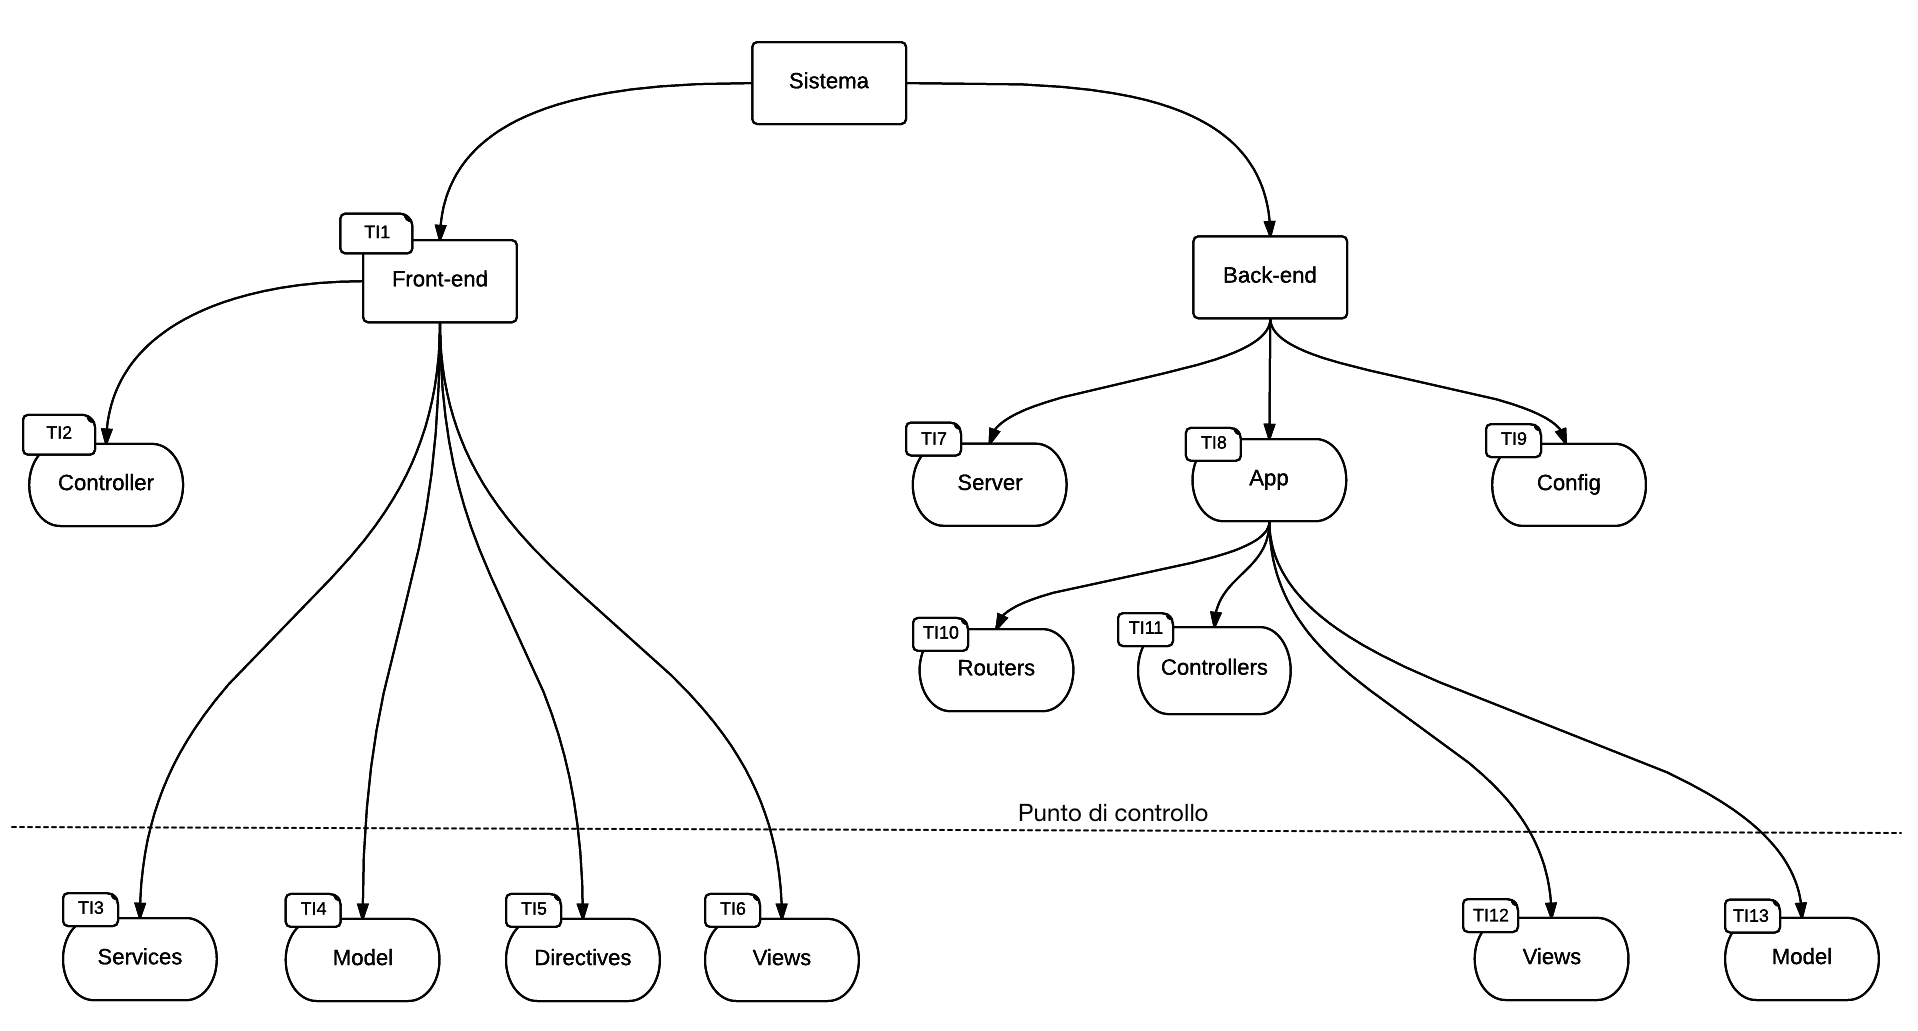
\includegraphics[scale=0.45,keepaspectratio]{Img/alberoTestIntegrazione.png}
\caption{Albero di integrazione delle componenti}
\end{figure}
\FloatBarrier
\end{center}
Nell'approccio top-down dei test di integrazione i moduli di livello più alto vengono sottoposti a test e integrati per primi. Così facendo anche la logica di alto livello e il flusso di dati vengono sottoposti a test fin da subito; sarà perciò necessario simulare le componenti di livello più basso con degli \gloxy{stub}. Una volta codificate, le componenti di più basso livello dovranno a loro volta essere integrate e testate. L'approccio top-down rientra tra le strategie di integrazione incrementali, che conferiscono il vantaggio di poter determinare in modo più immediato quale componente causa problemi: i difetti rilevati dai test, infatti, nella maggioranza dei casi saranno da attribuirsi all'ultima componente aggiunta.
\begin{center}
\begin{figure}[h]
\centering
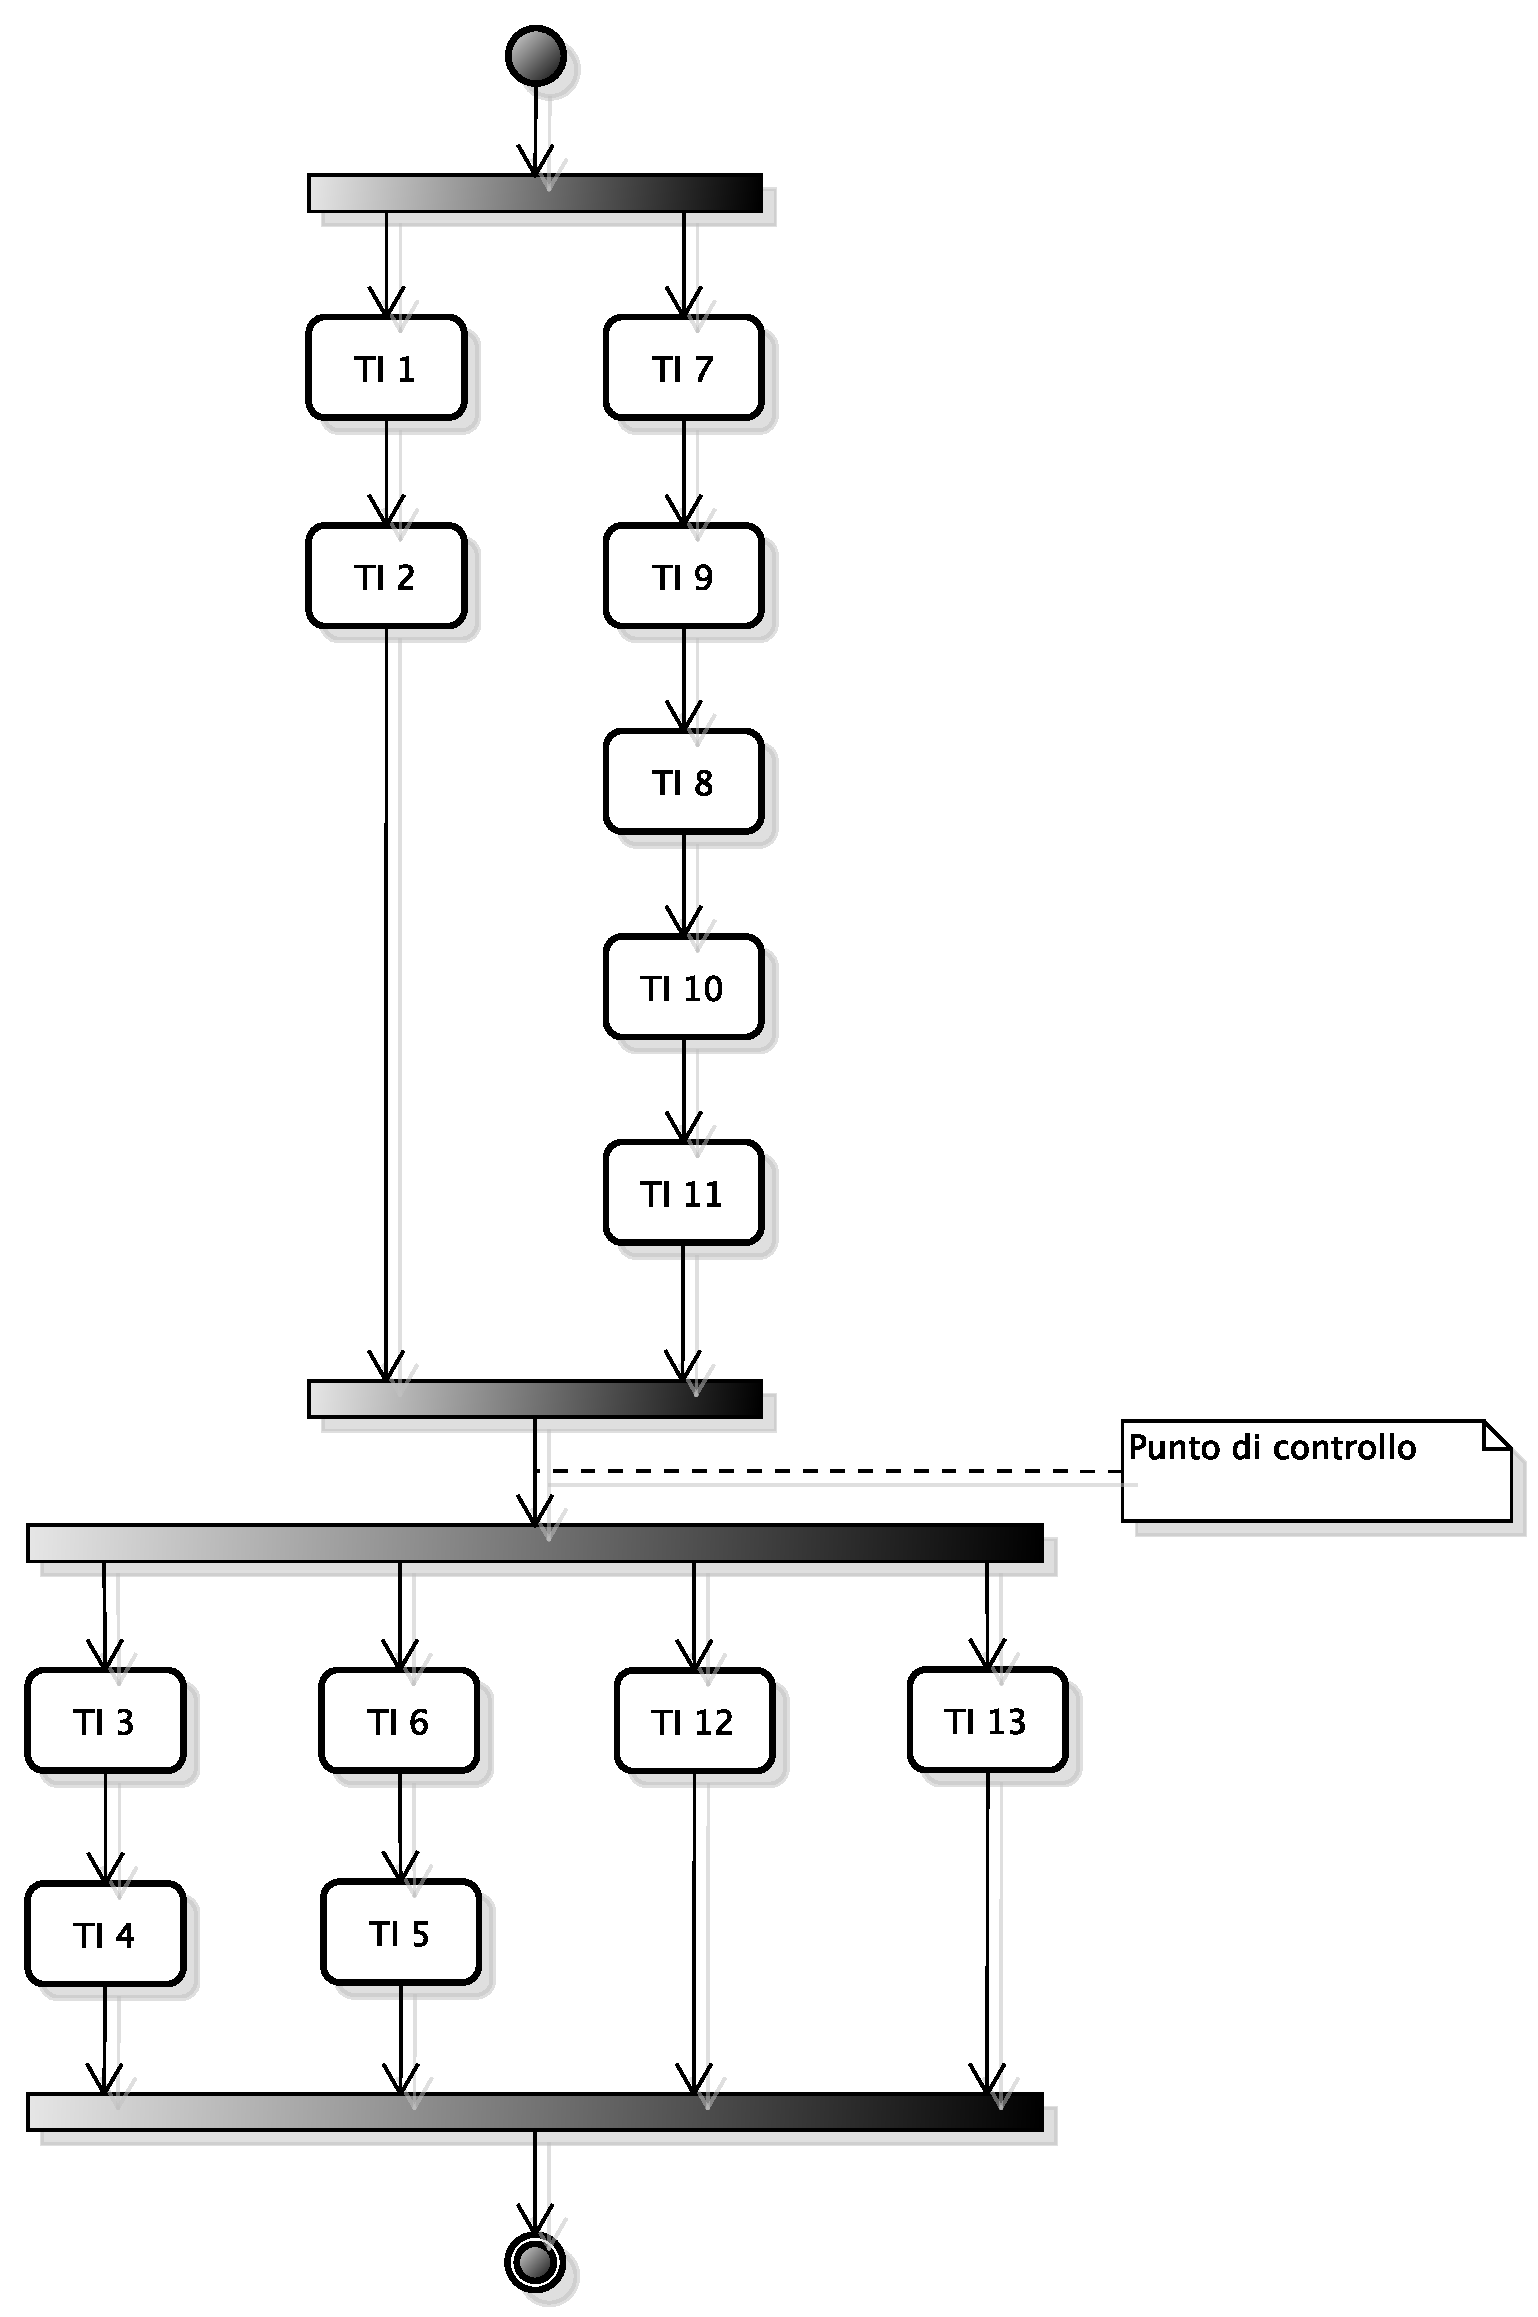
\includegraphics[scale=0.55,keepaspectratio]{Img/testIntegrazione.pdf}
\caption{Diagramma di attività dei test di integrazione}
\end{figure}
\FloatBarrier
\end{center}

\normalsize
\begin{longtable}{|c|>{}m{8cm}|c|}
\hline 
\textbf{Id Test} & \textbf{Descrizione} & \textbf{Stato}\\
\hline
\endhead
\hypertarget{TI1}{TI1} & Vengono verificate le dipendenze dei moduli del Front-End. & \textcolor{Green}{\textit{Superato}}\\ \hline
\hypertarget{TI2}{TI2} & Viene verificato che i \textit{Services} permettano di interagire correttamente con il Back-End. & \textit{Non Implementato}\\ \hline
\hypertarget{TI3}{TI3} & Viene verificato che i \textit{Services} si integrino correttamente fra loro. & \textcolor{Green}{\textit{Superato}}\\ \hline
\hypertarget{TI4}{TI4} & Viene verificato che i \textit{Controller} si integrino correttamente con i \textit{Services}. & \textit{Non Implementato}\\ \hline
\hypertarget{TI5}{TI5} & Viene verificato che il \textit{Model} si integri correttamente con i \textit{Services}. & \textcolor{Green}{\textit{Superato}}\\ \hline
\hypertarget{TI6}{TI6} & Viene verificato che il \textit{Model} si integri correttamente con i \textit{Controller}. & \textit{Non Implementato}\\ \hline
\hypertarget{TI7}{TI7} & Viene verificato che \textit{App} si integri correttamente con le librerie di Express e Node.js utilizzate. & \textcolor{Green}{\textit{Superato}}\\ \hline
\hypertarget{TI8}{TI8} & Viene verificato che \textit{Config} si integri con \textit{Server}, carichi correttamente tutte le librerie per Node.js che utilizzerà e che istanzi le classi del package \textit{App} in modo corretto. & \textcolor{Green}{\textit{Superato}}\\ \hline
\hypertarget{TI9}{TI9} & Viene verificato che i \textit{Routers} si integrino correttamente con il package \textit{App} e reindirizzino adeguatamente le richieste REST destinate al server. & \textcolor{Green}{\textit{Superato}}\\ \hline
\hypertarget{TI10}{TI10} & Viene verificato che i \textit{Controller} si integrino correttamente e gestiscano le richieste inoltrate dai \textit{Routers}. & \textcolor{Green}{\textit{Superato}}\\ \hline
\hypertarget{TI11}{TI11} & Viene verificato che le \textit{View} si integrino con i \textit{Controller} per fornire al Front-End pagine web statiche. & \textcolor{Green}{\textit{Superato}}\\ \hline
\hypertarget{TI12}{TI12} & Viene verificato che il \textit{Model} si integri correttamente con i \textit{Controller} per la gestione dell'inserimento, della modifica e dell'eliminazione dei dati. & \textit{Non Implementato}\\ \hline
\caption[Test di Integrazione]{Test di Integrazione}
\label{tabella:test2}
\end{longtable}
\clearpage

\subsection{Test di Unità}
Con questa tipologia di test si vuole verificare il corretto funzionamento delle unità individuate  durante la definizione dell'architettura ad alto livello.\\
I test di unità saranno descritti nel modo seguente:
\begin{center}
\textbf{TU}[\textit{IdTest}]
\end{center}
dove:
\begin{itemize}
\item \textbf{IdTest} rappresenta il codice identificativo crescente dell'unità considerata.
\end{itemize}

\normalsize
\begin{longtable}{|c|>{}m{8cm}|c|}
\hline 
\textbf{Id Test} & \textbf{Descrizione} & \textbf{Stato}\\
\hline
\endhead
\hypertarget{TU1}{TU1} & Verificare che l'istanza del server venga creata correttamente e che si metta in ascolto su \texttt{localhost:3333}\finaleTestUnita{}. & \textcolor{Green}{\textit{Superato}}\\ \hline
\hypertarget{TU2}{TU2} & Verificare che, ricevendo delle richieste conformi alle API definite, il metodo setti tutti i routes ed i middleware sui parametri, l'oggetto passi il controllo al \texttt{concreteHandler} corretto\finaleTestUnita{}. & \textcolor{Green}{\textit{Superato}}\\ \hline
\hypertarget{TU3}{TU3} & Verificare che, ricevendo delle richieste conformi alle API definite, il metodo setti tutti i routes, l'oggetto passi il controllo al \texttt{concreteHandler} corretto\finaleTestUnita{}. & \textcolor{Green}{\textit{Superato}}\\ \hline
\hypertarget{TU4}{TU4} & Verificare che, ricevendo delle richieste conformi alle API definite, il metodo setti tutti i routes, l'oggetto passi il controllo al \texttt{concreteHandler} corretto\finaleTestUnita{}. & \textcolor{Green}{\textit{Superato}}\\ \hline
\hypertarget{TU5}{TU5} & Verificare che, in base ai parametri forniti in input, il JSON ritornato contenga il messaggio d’errore corretto\finaleTestUnita{}. & \textcolor{Green}{\textit{Superato}}\\ \hline
\hypertarget{TU6}{TU6} & Verificare che, in base ai parametri forniti in input, il JSON ritornato contenga il messaggio d'errore corretto\finaleTestUnita{}. & \textcolor{Green}{\textit{Superato}}\\ \hline
\hypertarget{TU7}{TU7} & Verificare che, in base alle informazioni fornite in input, il metodo \textit{getter} setti in modo corretto i parametri correlati\finaleTestUnita{}. & \textcolor{Green}{\textit{Superato}}\\ \hline
\hypertarget{TU8}{TU8} & Verificare che il messaggio d'errore venga costruito in modo coerente rispetto ai dati passati al costruttore e che i metodi disponibili restituiscano l'informazione nel formato desiderato\finaleTestUnita{}. & \textcolor{Green}{\textit{Superato}}\\ \hline
\hypertarget{TU9}{TU9} & Verificare che, in base ai parametri forniti in input, i metodi effettuino le operazioni richieste, controllando l'esistenza dell'id del nodo o dell'id dell'associazione nel database\finaleTestUnita{}. & \textcolor{Green}{\textit{Superato}}\\ \hline
\hypertarget{TU10}{TU10} & Verificare che, in base ai parametri forniti in input, i metodi effettuino le operazioni richieste, mantenendo aggiornata la mappa aggiungendo o eliminando associazioni fra i nodi\finaleTestUnita{}. & \textcolor{Green}{\textit{Superato}}\\ \hline
\hypertarget{TU11}{TU11} & Verificare che, in base ai parametri forniti in input, i metodi effettuino le operazioni richieste, mantenendo aggiornata la mappa aggiungendo, eliminando o modificando i nodi\finaleTestUnita{}. & \textcolor{Green}{\textit{Superato}}\\ \hline
\hypertarget{TU12}{TU12} & Verificare che, in base ai parametri forniti in input, il metodo effettui le operazioni richieste, controllando l'esistenza dell'id del percorso di presentazione nel database\finaleTestUnita{}. & \textcolor{Green}{\textit{Superato}}\\ \hline
\hypertarget{TU13}{TU13} & Verificare che, in base ai parametri forniti in input, i metodi effettuino le operazioni richieste, mantenendo aggiornati i percorsi di presentazione\finaleTestUnita{}. & \textcolor{Green}{\textit{Superato}}\\ \hline
\hypertarget{TU14}{TU14} & Verificare che, in base ai parametri forniti in input, il metodo effettui le operazioni richieste, controllando che il progetto con \texttt{id} specificato esista\finaleTestUnita{}. & \textcolor{Green}{\textit{Superato}}\\ \hline
\hypertarget{TU15}{TU15} & Verificare che, in base ai parametri forniti in input, i metodi effettuino le operazioni richieste, restituendo i percorsi di presentazione, completi di tutte le informazioni necessarie ad eseguire una presentazione, eliminando il progetto specificato\finaleTestUnita{}. & \textcolor{Green}{\textit{Superato}}\\ \hline
\hypertarget{TU16}{TU16} & Verificare che, in base ai parametri forniti in input, i metodi effettuino le operazioni richieste, creando un nuovo progetto, modificando un progetto esistente, ottenendo tutti i progetti dell'utente e tutte le informazioni relative ad un dato progetto, in particolare la sua mappa mentale\finaleTestUnita{}. & \textcolor{Green}{\textit{Superato}}\\ \hline
\hypertarget{TU17}{TU17} & Verificare che, in base ai parametri forniti in input, i metodi effettuino le operazioni richieste, mantenendo aggiornate le informazioni riguardanti registrazione ed autenticazione dell’utente\finaleTestUnita{}. & \textcolor{Green}{\textit{Superato}}\\ \hline
\hypertarget{TU18}{TU18} & Verificare che, in base ai parametri forniti in input, il metodo effettui le operazioni richieste, verificando che l'utente che esegue la richiesta sia effettivamente un utente autenticato e  mantenendo aggiornate le informazioni riguardanti l'identificazione dell’utente\finaleTestUnita{}. & \textcolor{Green}{\textit{Superato}}\\ \hline
\hypertarget{TU19}{TU19} & Verificare che, dato in input un JSON formattato correttamente, il metodo restituisca un JSON corretto contenente le informazioni richieste riguardanti il contenuto di un nodo\finaleTestUnita{}. & \textcolor{Green}{\textit{Superato}}\\ \hline
\hypertarget{TU20}{TU20} & Verificare che, in base ai parametri forniti in input, i metodi effettuino le operazioni richieste, mantenendo aggiornate le informazioni del nodo in modo corretto, creando un nuovo nodo, aggiornandone il contenuto e restituendone le informazioni nel relativo JSON\finaleTestUnita{}. & \textcolor{Green}{\textit{Superato}}\\ \hline
\hypertarget{TU21}{TU21} & Verificare che, in base ai parametri forniti in input, il metodo crei un'istanza di \texttt{PathModel} che rappresenta il percorso di presentazione di default per il progetto, restituisca il relativo JSON\finaleTestUnita{}. & \textcolor{Green}{\textit{Superato}}\\ \hline
\hypertarget{TU22}{TU22} & Verificare che, in base ai parametri forniti in input, il metodo crei un'istanza di \texttt{PathModel} che rappresenta un percorso di presentazione personalizzato per il progetto, restituisca il relativo JSON\finaleTestUnita{}. & \textcolor{Green}{\textit{Superato}}\\ \hline
\hypertarget{TU23}{TU23} & Verificare che, in base ai parametri forniti in input, i metodi effettuino le operazioni richieste, mantenendo aggiornate le informazioni dell'istanza di \texttt{PathModel} in modo corretto, aggiungendo e rimuovendo nodi dal percorso di presentazione e rinominando il percorso stesso, che restituiscano il relativo JSON\finaleTestUnita{}. & \textcolor{Green}{\textit{Superato}}\\ \hline
\hypertarget{TU24}{TU24} & Verificare che, in base ai parametri forniti in input, il metodo crei un nuovo progetto, completo di mappa mentale e di un percorso di presentazione di default con un nodo preesistente, restituisca il relativo JSON\finaleTestUnita{}. & \textcolor{Green}{\textit{Superato}}\\ \hline
\hypertarget{TU25}{TU25} & Verificare che, in base ai parametri forniti in input, i metodi effettuino le operazioni richieste, mantenendo aggiornati i parametri di layout del progetto in modo corretto, restituiscano il relativo JSON\finaleTestUnita{}. & \textcolor{Green}{\textit{Superato}}\\ \hline
\hypertarget{TU26}{TU26} & Verificare che, in base ai parametri forniti in input, i metodi effettuino le operazioni richieste, aggiungendo e modificando nodi del progetto e restituendo i dati aggiornati in JSON\finaleTestUnita{}. & \textcolor{Green}{\textit{Superato}}\\ \hline
\hypertarget{TU27}{TU27} & Verificare che, in base ai parametri forniti in input, il metodo effettui le operazioni richieste, rimuovendo nodi dal progetto e dai percorsi di presentazione in cui erano inclusi, rimuovendo le associazioni ad essi correlate e restituendo i dati aggiornati in JSON\finaleTestUnita{}. & \textcolor{Green}{\textit{Superato}}\\ \hline
\hypertarget{TU28}{TU28} & Verificare che, in base ai parametri forniti in input, i metodi effettuino le operazioni richieste, aggiungendo e rimuovendo associazioni fra i nodi e restituendo i dati aggiornati in JSON\finaleTestUnita{}. & \textcolor{Green}{\textit{Superato}}\\ \hline
\hypertarget{TU29}{TU29} & Verificare che, in base ai parametri forniti in input, i metodi effettuino le operazioni richieste, aggiungendo, rinominando, rimuovendo percorsi di presentazione e aggiungendo, rimuovendo nodi da tali percorsi e restituendo i dati aggiornati in JSON\finaleTestUnita{}. & \textcolor{Green}{\textit{Superato}}\\ \hline
\hypertarget{TU30}{TU30} & Verificare che, in base ai parametri forniti in input, i metodi effettuino le operazioni richieste, restituendo in JSON la lista dei percorsi e la lista dei nodi di un percorso specifico\finaleTestUnita{}. & \textcolor{Green}{\textit{Superato}}\\ \hline
\hypertarget{TU31}{TU31} & Verificare che, all'inizializzazione dell'applicazione, la collection \texttt{relations} sia vuota e che, in base ai parametri forniti in input, il metodo effettui le operazioni richieste, costruendo in modo corretto \textit{relazioni gerarchiche} ed \textit{associazioni}  e  restituendo i dati aggiornati in JSON\finaleTestUnita{}. & \textcolor{Green}{\textit{Superato}}\\ \hline
\hypertarget{TU32}{TU32} & Verificare che, all'inizializzazione dell'applicazione, la collection \texttt{users} sia vuota e che, in base ai parametri forniti in input, il metodo effettui le operazioni richieste, costruendo un nuovo oggetto \texttt{Utente}, oppure restituendo opportuni avvisi nel caso in cui non siano stati inseriti tutti i parametri secondo indicazione o nel caso in cui la mail sia già stata utilizzata per un altro account e  restituendo i dati aggiornati in JSON\finaleTestUnita{}. & \textcolor{Green}{\textit{Superato}}\\ \hline
\hypertarget{TU33}{TU33} & Verificare che il metodo effettui le operazioni richieste, costruendo l’oggetto corrispondente e, per mezzo di \texttt{\$routeProvider}, associando ad ogni route un controller ed una view\finaleTestUnita{}. & \textcolor{Green}{\textit{Superato}}\\ \hline
\hypertarget{TU34}{TU34} & Verificare che, in base ai parametri forniti in input, i metodi effettuino le operazioni richieste, costruendo l'oggetto gestore della directive \texttt{premiAddToPath}, restituendo se il bottone di conferma è abilitato, gestendo correttamente gli eventi di click dei pulsanti di conferma ed annullamento dell'operazione di inserimento di un nodo nel percorso di presentazione\finaleTestUnita{}. & \textcolor{Green}{\textit{Superato}}\\ \hline
\hypertarget{TU35}{TU35} & Verificare che, in base ai parametri forniti in input, i metodi effettuino le operazioni richieste, costruendo l'oggetto gestore della directive \texttt{premiAssociationAdder}, restituendo se il bottone di conferma è abilitato, gestendo correttamente gli eventi di click dei pulsanti di conferma ed annullamento dell'operazione di inserimento di un'associazione\finaleTestUnita{}. & \textcolor{Green}{\textit{Superato}}\\ \hline
\hypertarget{TU36}{TU36} & Verificare che, in base ai parametri forniti in input, i metodi effettuino le operazioni richieste, invocando correttamente la funzione \texttt{callback} del parametro \texttt{fn}, nascondendo il menù per mezzo del metodo \texttt{\$mdDialog.cancel}\finaleTestUnita{}. & \textcolor{Green}{\textit{Superato}}\\ \hline
\hypertarget{TU37}{TU37} & Verificare che, in base ai parametri forniti in input, il metodo effettui le operazioni richieste, creando l'oggetto corrispondente e popolando lo \texttt{\$scope} nel modo atteso\finaleTestUnita{}. & \textcolor{Green}{\textit{Superato}}\\ \hline
\hypertarget{TU38}{TU38} & Verificare che, in base ai parametri forniti in input, i metodi effettuino le operazioni richieste, aggiornando i progetti dell'utente, che \texttt{\$scope} venga modificato nel modo atteso e che, in caso di caricamento di altre view, venga effettuata correttamente la chiamata a \texttt{\$location}\finaleTestUnita{}. & \textcolor{Green}{\textit{Superato}}\\ \hline
\hypertarget{TU39}{TU39} & Verificare che, in base ai parametri forniti in input, i metodi effettuino le operazioni richieste, costruendo l'oggetto gestore della directive \texttt{premiEditableNodeContent}, gestendo correttamente la selezione del contenuto di un nodo sollevando l'evento \texttt{nodecontent-selected} e fornendo l'\texttt{id} dell'oggetto \texttt{NodeContent}\finaleTestUnita{}. & \textcolor{Green}{\textit{Superato}}\\ \hline
\hypertarget{TU40}{TU40} & Verificare che, in base ai parametri forniti in input, il metodo effettui le operazioni richieste, nascondendo la directive \texttt{premiErrorMessage}\finaleTestUnita{}. & \textcolor{Green}{\textit{Superato}}\\ \hline
\hypertarget{TU41}{TU41} & Verificare che, in base ai parametri forniti in input, il metodo effettui le operazioni richieste, costruendo l'oggetto gestore della directive \texttt{premiHeader} in modo corretto\finaleTestUnita{}. & \textcolor{Green}{\textit{Superato}}\\ \hline
\hypertarget{TU42}{TU42} & Verificare che, in base ai parametri forniti in input, i metodi effettuino le operazioni richieste, controllando se l'URL corrente contiene la stringa ricevuta come parametro, ritornando il titolo da visualizzare, mostrando il manuale utente, invertendo il valore del campo dati \texttt{sidenavOpen}, adattando le dimensioni della mappa mentale e permettendo di regolare lo zoom su di essa\finaleTestUnita{}. & \textcolor{Green}{\textit{Superato}}\\ \hline
\hypertarget{TU43}{TU43} & Verificare che, in base ai parametri forniti in input, i metodi effettuino le operazioni richieste, reindirizzando l'utente alla view identificata dall'URL ricevuto come parametro, visualizzando la directive per la modifica delle impostazioni del progetto, invocando la funzionalità di stampa del browser, gestendo gli eventi \texttt{click} sul pulsante per modificare la mappa mentale, sul pulsante per modificare i percorsi di presentazione, sul pulsante di logout\finaleTestUnita{}. & \textcolor{Green}{\textit{Superato}}\\ \hline
\hypertarget{TU44}{TU44} & Verificare che, in base ai parametri forniti in input, i metodi effettuino le operazioni richieste, costruendo l'oggetto gestore della visibilità della directive \texttt{premiHierarchicalMenu}, rendendo visibile o nascondendo la directive\finaleTestUnita{}. & \textcolor{Green}{\textit{Superato}}\\ \hline
\hypertarget{TU45}{TU45} & Verificare che, in base ai parametri forniti in input, i metodi effettuino le operazioni richieste, costruendo l'oggetto gestore della logica applicativa del \textit{login}, verificando se è già presente una sessione, recuperando i dati dallo \$scope ed effettuando l'autenticazione (utilizzando \texttt{AuthenticationService}), effettuando il redirect verso la pagina di registrazione\finaleTestUnita{}. & \textcolor{Green}{\textit{Superato}}\\ \hline
\hypertarget{TU46}{TU46} & Verificare che, in base ai parametri forniti in input, il metodo effettui le operazioni richieste, creando l'oggetto corrispondente e popolando lo \texttt{\$scope} nel modo atteso\finaleTestUnita{}. & \textcolor{Green}{\textit{Superato}}\\ \hline
\hypertarget{TU47}{TU47} & Verificare che, in base ai parametri forniti in input, i metodi effettuino le operazioni richieste, editando la mappa secondo le indicazioni e popolando lo \texttt{\$scope} nel modo atteso\finaleTestUnita{}. & \textcolor{Green}{\textit{Superato}}\\ \hline
\hypertarget{TU48}{TU48} & Verificare che i metodi effettuino le operazioni richieste, resettando l'elemento desiderato, scegliendo di editare il nodo, iniziando ad aggiungere una nuova associazione e aggiornando lo \texttt{\$scope} nel modo atteso\finaleTestUnita{}. & \textcolor{Green}{\textit{Superato}}\\ \hline
\hypertarget{TU49}{TU49} & Verificare che, in base ai parametri forniti in input, i metodi effettuino le operazioni richieste, costruendo l'oggetto gestore della logica legata alla modifica del contenuto di un nodo, aggiungendo o rimuovendo elementi (come immagini e testo), gestendo gli eventi \texttt{click} di conferma o annullamento delle modifiche e di selezione di una slide\finaleTestUnita{}. & \textcolor{Green}{\textit{Superato}}\\ \hline
\hypertarget{TU50}{TU50} & Verificare che, in base ai parametri forniti in input, il metodo effettui le operazioni richieste, costruendo l'oggetto gestore della directive \texttt{premiNode}, utilizzato per gestire lo stile di visualizzazione del frame che deve essere visualizzato dalla directive\finaleTestUnita{}. & \textcolor{Green}{\textit{Superato}}\\ \hline
\hypertarget{TU51}{TU51} & Verificare che, in base ai parametri forniti in input, i metodi effettuino le operazioni richieste, costruendo l'oggetto gestore della logica e della visibilità della directive \texttt{premiPath}, rimuovendo un nodo dal percorso di presentazione, salvando le modifiche attuate\finaleTestUnita{}. & \textcolor{Green}{\textit{Superato}}\\ \hline
\hypertarget{TU52}{TU52} & Verificare che, in base ai parametri forniti in input, i metodi effettuino le operazioni richieste, costruendo l'oggetto gestore dei percorsi di presentazione\finaleTestUnita{}. & \textcolor{Green}{\textit{Superato}}\\ \hline
\hypertarget{TU53}{TU53} & Verificare che, in base ai parametri forniti in input, i metodi effettuino le operazioni richieste, impostando il percorso corrente come riferimento al parametro \texttt{path}, deselezionando il percorso di presentazione precedentemente selezionato\finaleTestUnita{}. & \textcolor{Green}{\textit{Superato}}\\ \hline
\hypertarget{TU54}{TU54} & Verificare che, in base ai parametri forniti in input, i metodi effettuino le operazioni richieste, utilizzando opportunamente \texttt{PathService} per creare un nuovo percorso di presentazione, rimuoverne uno già definito, confermare la selezione e avviare la presentazione di un percorso specifico\finaleTestUnita{}. & \textcolor{Green}{\textit{Superato}}\\ \hline
\hypertarget{TU55}{TU55} & Verificare che, in base ai parametri forniti in input, i metodi effettuino le operazioni richieste, costruendo l'oggetto gestore della logica applicativa della presentazione di un percorso, visualizzando la slide precedente e quella successiva\finaleTestUnita{}. & \textit{Non Implementato}\\ \hline
\hypertarget{TU56}{TU56} & Verificare che, in base ai parametri forniti in input, il metodo effettui le operazioni richieste, costruendo l'oggetto gestore della logica applicativa riguardante l’esecuzione di un percorso di presentazione\finaleTestUnita{}. & \textcolor{Green}{\textit{Superato}}\\ \hline
\hypertarget{TU57}{TU57} & Verificare che, in base ai parametri forniti in input, i metodi effettuino le operazioni richieste, permettendo di passare da un frame ad un frame correlato, emettendo l'evento \texttt{presentation-previousStep} al passaggio al frame precedente e \texttt{presentation-nextStep} al passaggio al frame successivo, aggiornando le informazioni al cambio del nodo, visualizzando la pagina di stampa, permettendo di ripristinare la presentazione lineare\finaleTestUnita{}. & \textcolor{Green}{\textit{Superato}}\\ \hline
\hypertarget{TU58}{TU58} & Verificare che, in base ai parametri forniti in input, i metodi effettuino le operazioni richieste, terminando la presentazione e rinviando l'utente alla pagina iniziale o alla pagina per la modifica dei percorsi di presentazione, attivando o disattivando la modalità a schermo intero, mostrando il manuale, invertendo il valore del campo dati \texttt{sidenavOpen}\finaleTestUnita{}. & \textcolor{Green}{\textit{Superato}}\\ \hline
\hypertarget{TU59}{TU59} & Verificare che, in base ai parametri forniti in input, i metodi effettuino le operazioni richieste, costruendo l'oggetto gestore della logica di funzionamento della directive \texttt{premiProjectSettingsEditor}, aggiornando l'anteprima dello stile del progetto, gestendo gli eventi generati dal click dei tasti per salvare o dimenticare le modifiche apportate\finaleTestUnita{}. & \textcolor{Green}{\textit{Superato}}\\ \hline
\hypertarget{TU60}{TU60} & Verificare che, in base ai parametri forniti in input, i metodi effettuino le operazioni richieste, gestendo la cancellazione di un progetto dalla lista dei progetti (previa conferma dell'operazione), rendendo visibile la finestra di dialogo per la scelta del percorso di presentazione da presentare\finaleTestUnita{}. & \textcolor{Green}{\textit{Superato}}\\ \hline
\hypertarget{TU61}{TU61} & Verificare che, in base ai parametri forniti in input, i metodi effettuino le operazioni richieste, costruendo l'oggetto gestore della logica di funzionamento della registrazione di un utente, utilizzando \texttt{AuthenticationService} per registrare un nuovo utente in caso di conferma, effettuando il redirect verso la pagina di \textit{login}\finaleTestUnita{}. & \textcolor{Green}{\textit{Superato}}\\ \hline
\hypertarget{TU62}{TU62} & Verificare che, in base ai parametri forniti in input, i metodi effettuino le operazioni richieste, costruendo l'oggetto gestore della visibilità della directive \texttt{premiSmartMenu}, rendendo visibile o nascondendo la directive\finaleTestUnita{}. & \textcolor{Green}{\textit{Superato}}\\ \hline
\hypertarget{TU63}{TU63} & Verificare che, in base ai parametri forniti in input, i metodi effettuino le operazioni richieste, costruendo l'oggetto contenente le informazioni sull'errore, ritornando correttamente il titolo, il messaggio ed il codice dell'errore\finaleTestUnita{}. & \textcolor{Green}{\textit{Superato}}\\ \hline
\hypertarget{TU64}{TU64} & Verificare che i metodi \textit{getter} effettuino le operazioni richieste, restituendo le informazioni sul nodo desiderato\finaleTestUnita{}. & \textcolor{Green}{\textit{Superato}}\\ \hline
\hypertarget{TU65}{TU65} & Verificare che, in base ai parametri forniti in input, i metodi effettuino le operazioni richieste, impostando e/o eliminando parte del contenuto del nodo desiderato\finaleTestUnita{}. & \textcolor{Green}{\textit{Superato}}\\ \hline
\hypertarget{TU66}{TU66} & Verificare che, in base ai parametri forniti in input, i metodi effettuino le operazioni richieste, creando l'oggetto corrispondente, settando il contenuto del nodo nel modo atteso e restituendo le informazioni in esso contenute\finaleTestUnita{}. & \textcolor{Green}{\textit{Superato}}\\ \hline
\hypertarget{TU67}{TU67} & Verificare che, in base ai parametri forniti in input, i metodi effettuino le operazioni richieste, settando le informazioni relative al nodo\finaleTestUnita{}. & \textcolor{Green}{\textit{Superato}}\\ \hline
\hypertarget{TU68}{TU68} & Verificare che i metodi \textit{getter} effettuino le operazioni richieste, restituendo le informazioni su un passo del percorso di presentazione desiderato\finaleTestUnita{}. & \textcolor{Green}{\textit{Superato}}\\ \hline
\hypertarget{TU69}{TU69} & Verificare che, in base ai parametri forniti in input, i metodi effettuino le operazioni richieste, aggiungendo ed eliminando un passo di presentazione dal percorso di presentazione desiderato prestabilito\finaleTestUnita{}. & \textcolor{Green}{\textit{Superato}}\\ \hline
\hypertarget{TU70}{TU70} & Verificare che i metodi \textit{getter} effettuino le operazioni richieste, restituendo le informazioni sugli attributi del percorso di presentazione desiderato\finaleTestUnita{}. & \textcolor{Green}{\textit{Superato}}\\ \hline
\hypertarget{TU71}{TU71} & Verificare che, in base ai parametri forniti in input, il metodo effettui le operazioni richieste, settando il nome del percorso di presentazione desiderato, verificando se è il percorso di presentazione di default\finaleTestUnita{}. & \textcolor{Green}{\textit{Superato}}\\ \hline
\hypertarget{TU72}{TU72} & Verificare che i metodi \textit{getter} effettuino le operazioni richieste, restituendo le informazioni sui nodi associati a quello desiderato\finaleTestUnita{}. & \textcolor{Green}{\textit{Superato}}\\ \hline
\hypertarget{TU73}{TU73} & Verificare che i metodi \textit{getter} effettuino le operazioni richieste, restituendo le informazioni sul progetto corrente\finaleTestUnita{}. & \textcolor{Green}{\textit{Superato}}\\ \hline
\hypertarget{TU74}{TU74} & Verificare che, in base ai parametri forniti in input, i metodi \textit{setter} effettuino le operazioni richieste, settando le informazioni del progetto corrente\finaleTestUnita{}. & \textcolor{Green}{\textit{Superato}}\\ \hline
\hypertarget{TU75}{TU75} & Verificare che, in base ai parametri forniti in input, utilizzando il service \texttt{\$http}, i metodi effettuino le richieste riguardanti l’autenticazione al backend in maniera corretta, che i dati vengano restituiti nella maniera attesa\finaleTestUnita{}. & \textcolor{Green}{\textit{Superato}}\\ \hline
\hypertarget{TU76}{TU76} & Verificare che, in base ai parametri forniti in input, i metodi si occupino di esaudire le modifiche richieste utilizzando le funzionalità offerte da \textit{Cytoscape.js}, che i dati vengano restituiti nella maniera attesa\finaleTestUnita{}. & \textit{Non Implementato}\\ \hline
\hypertarget{TU77}{TU77} & Verificare, utilizzando il service \texttt{\$httpBackend} fornito da \textit{Angular.js}, che, in base ai parametri forniti in input, i metodi richiedano  in maniera corretta l’aggiornamento delle informazioni inerenti la mappa mentale sia al backend che in locale, utilizzando i service \texttt{\$http} e \texttt{MindmapAdapterService}, che i dati vengano restituiti nella maniera attesa\finaleTestUnita{}. & \textcolor{Green}{\textit{Superato}}\\ \hline
\hypertarget{TU78}{TU78} & Verificare che, in base ai parametri forniti in input, utilizzando il service \texttt{MindmapAdapterService}, i metodi richiedano in maniera corretta l’aggiornamento delle informazioni inerenti la mappa mentale in locale, che i dati vengano restituiti nella maniera attesa\finaleTestUnita{}. & \textcolor{Green}{\textit{Superato}}\\ \hline
\hypertarget{TU79}{TU79} & Verificare, utilizzando il service \texttt{\$httpBackend} fornito da \textit{Angular.js}, che, in base ai parametri forniti in input, i metodi richiedano in maniera corretta l'aggiornamento delle informazioni inerenti il percorso di presentazione al backend, utilizzando il service \texttt{\$http}, che i dati vengano restituiti nella maniera attesa\finaleTestUnita{}. & \textcolor{Green}{\textit{Superato}}\\ \hline
\hypertarget{TU80}{TU80} & Verificare, utilizzando il service \texttt{\$httpBackend} fornito da \textit{Angular.js}, che, in base ai parametri forniti in input, i metodi \textit{getter} richiedano in maniera corretta le informazioni inerenti il percorso di presentazione al backend, utilizzando il service \texttt{\$http}, che i dati vengano restituiti nella maniera attesa\finaleTestUnita{}. & \textit{Non Implementato}\\ \hline
\hypertarget{TU81}{TU81} & Verificare, utilizzando il service \texttt{\$httpBackend} fornito da \textit{Angular.js}, che, in base ai parametri forniti in input, i metodi richiedano in maniera corretta l’aggiornamento delle informazioni inerenti i progetti creati dall’utente, utilizzando il service \texttt{\$http}, che i dati vengano restituiti nella maniera attesa\finaleTestUnita{}. & \textcolor{Green}{\textit{Superato}}\\ \hline
\caption[Test di Unità]{Test di Unità}
\label{tabella:test3}
\end{longtable}
\clearpage

